% ---------------------------------------------------------------------------
% A twenty-minute lecture in the OpenCode design language: warm cream canvas,
% monospaced type, hairline rules, ASCII markers, one dark card.
% Every number is measured on a 102M-parameter network trained on 4.2 GB text.
% Build: xelatex slides.tex   (twice, for the page counter)
% ---------------------------------------------------------------------------
\documentclass[aspectratio=169,11pt]{beamer}

\usepackage{fontspec}
\usepackage{unicode-math}
\setmainfont{Noto Sans Mono}[
  UprightFont = *-Regular, BoldFont = *-Bold, ItalicFont = *-Regular,
  Ligatures = NoCommon]
\setmonofont{Noto Sans Mono}[Ligatures = NoCommon]
\setsansfont{Noto Sans Mono}[Ligatures = NoCommon]
\setmathfont{Latin Modern Math}
\setmathfont{Noto Sans Math}[range={up/{Latin,latin,Greek,greek},sfup/{Latin,latin,Greek,greek}}]

\usepackage{booktabs}
\usepackage{graphicx}
\usepackage{tikz}
\usetikzlibrary{arrows.meta,calc,positioning}

% ------------------------------------------------------------- the palette
\definecolor{canvas}{HTML}{FDFCFC}
\definecolor{ink}{HTML}{201D1D}
\definecolor{inkdeep}{HTML}{0F0000}
\definecolor{bodyink}{HTML}{424245}
\definecolor{mute}{HTML}{646262}
\definecolor{stone}{HTML}{6E6E73}
\definecolor{ash}{HTML}{9A9898}
\definecolor{card}{HTML}{F1EEEE}
\definecolor{dark}{HTML}{201D1D}
\definecolor{darkelev}{HTML}{302C2C}
\definecolor{hairline}{HTML}{E7E3E3}
\definecolor{accent}{HTML}{007AFF}
\definecolor{danger}{HTML}{FF3B30}
\definecolor{warning}{HTML}{FF9F0A}
\definecolor{success}{HTML}{30D158}

% ------------------------------------------------------------------- setup
\setbeamertemplate{navigation symbols}{}
\setbeamercolor{normal text}{fg=ink,bg=canvas}
\setbeamercolor{structure}{fg=accent}
\setbeamertemplate{background canvas}{\color{canvas}\vrule width\paperwidth height\paperheight}

\setbeamerfont{frametitle}{size=\Large,series=\bfseries}
\setbeamerfont{title}{size=\Huge,series=\bfseries}
\setbeamerfont{itemize/enumerate body}{size=\normalsize}

\setbeamertemplate{itemize item}{\textcolor{accent}{\ttfamily [+]}}
\setbeamertemplate{itemize subitem}{\textcolor{mute}{\ttfamily [-]}}
\setlength{\leftmargini}{1.6em}
\setbeamertemplate{itemize/enumerate body begin}{\color{bodyink}}

% Title block: a hairline above, small mono kicker, then the claim.
\setbeamertemplate{frametitle}{%
  \vspace*{2pt}
  \hspace*{1pt}{\ttfamily\scriptsize\color{stone}\MakeUppercase{\insertframenumber}\ /\ 10}\par
  \vspace{5pt}
  \hspace*{1pt}{\usebeamerfont{frametitle}\color{ink}\insertframetitle}\par
  \vspace{4pt}
  \hspace*{1pt}{\color{hairline}\rule{\textwidth}{0.6pt}}%
  \vspace{2pt}
}

\setbeamertemplate{footline}{%
  \hspace*{14pt}{\ttfamily\tiny\color{ash}the rank of a matrix, and what it costs}\hfill
  {\ttfamily\tiny\color{ash}\insertframenumber\,/\,10}\hspace*{14pt}\vspace{6pt}}

\newcommand{\hl}[1]{{\color{accent}#1}}
\newcommand{\bad}[1]{{\color{danger}#1}}
\newcommand{\kick}[1]{{\ttfamily\scriptsize\color{stone}\textls[80]{\MakeUppercase{#1}}}}
\newcommand{\ascii}{\textcolor{accent}{\ttfamily [+]}}
\newcommand{\kv}[2]{\textcolor{mute}{#1}\,\textcolor{ink}{#2}}

\renewcommand{\familydefault}{\ttdefault}
\begin{document}

% ============================================================== 01 title
\setbeamertemplate{footline}{}
\begin{frame}[plain]
  \vspace{1.1cm}
  \hspace*{2pt}\kick{linear algebra \quad·\quad twenty minutes}
  \vspace{10pt}

  \hspace*{2pt}{\usebeamerfont{title}\color{ink}
    A matrix can be replaced\\[3pt]
    by two thin ones\par}

  \vspace{14pt}
  \hspace*{2pt}{\color{accent}\rule{2.4cm}{1.4pt}}

  \vspace{14pt}
  \hspace*{2pt}{\large\color{bodyink}
    Eckart--Young says how much you lose.\\[2pt]
    It does not say what you lose it \emph{for}.\par}

  \vfill
  \hspace*{2pt}
  \begin{minipage}{0.62\textwidth}
    \ttfamily\scriptsize\color{mute}
    measured on a 102\,678\,943-parameter network\\
    trained on 4.2 GB of text\quad·\quad four weight matrices\quad·\quad three seeds
  \end{minipage}
  \vspace{0.55cm}
\end{frame}

% ============================================================== 02 geometry
\begin{frame}{A weight matrix is a shape}
  \vspace{2pt}
  {\color{bodyink}
  A matrix $W\in\mathbb{R}^{m\times n}$ is a linear map. The honest picture is
  geometric: it sends the unit sphere to an \hl{ellipsoid}.\par}

  \vspace{4pt}
  \begin{center}
  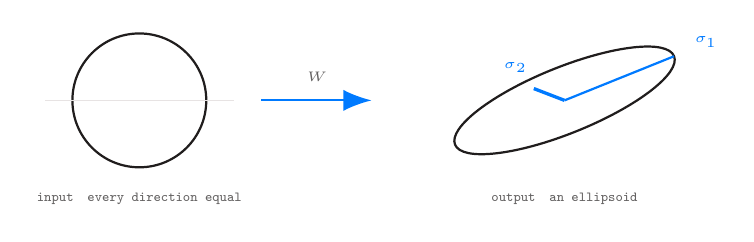
\begin{tikzpicture}[scale=1.0]
    \draw[ink,thick] (0,0) circle (0.85);
    \draw[hairline] (-1.2,0) -- (1.2,0);
    \node[below=3pt,font=\ttfamily\tiny,color=mute] at (0,-0.95) {input\quad every direction equal};
    \draw[-{Latex[length=3.6mm]},accent,thick] (1.55,0) -- (2.95,0);
    \node[above=3pt,font=\ttfamily\tiny,color=mute] at (2.25,0) {$W$};
    \begin{scope}[xshift=5.4cm]
      \draw[ink,thick,rotate=22] (0,0) ellipse (1.5 and 0.42);
      \draw[accent,thick] (0,0) -- (1.39,0.56);
      \node[font=\ttfamily\tiny,color=accent] at (1.80,0.74) {$\sigma_1$};
      \draw[accent,line width=1.2pt] (0,0) -- (-0.39,0.15);
      \node[font=\ttfamily\tiny,color=accent] at (-0.62,0.42) {$\sigma_2$};
      \node[below=3pt,font=\ttfamily\tiny,color=mute] at (0,-0.95) {output\quad an ellipsoid};
    \end{scope}
  \end{tikzpicture}
  \end{center}

  \vspace{2pt}
  {\ttfamily\scriptsize\color{stone}
  the semi-axes are the singular values --- geometry, before any learning}
\end{frame}

% ============================================================== 03 SVD
\begin{frame}{The decomposition is a sentence}
  \vspace{6pt}
  \[
    W \;=\; U\,\Sigma\,V^{\top},
    \qquad \Sigma=\operatorname{diag}(\sigma_1\ge\sigma_2\ge\cdots\ge0)
  \]
  \vspace{2pt}

  {\small\color{bodyink}
  \begin{tabular}{@{}p{2.6cm}p{7.4cm}@{}}
    \toprule
    \textcolor{mute}{factor} & \textcolor{mute}{what it does} \\
    \midrule
    $V^{\top}$ & turns the input onto the principal axes \\
    $\Sigma$   & stretches axis $i$ by $\sigma_i$ \\
    $U$        & turns the result into output space \\
    \bottomrule
  \end{tabular}}

  \vspace{10pt}
  {\color{bodyink}
  \hl{Rotate, stretch, rotate.} The $\sigma_i$ say \emph{how much} the map does in
  each direction --- and the natural hope is that most of them say
  \emph{almost nothing}.\par}

  \vspace{6pt}
  {\ttfamily\scriptsize\color{stone}
  that hope is the entire economic case for low-rank compression}
\end{frame}

% ============================================================== 04 theorem
\begin{frame}{Eckart--Young, 1936}
  \vspace{2pt}
  {\small\color{bodyink}Let $W_r=\sum_{i\le r}\sigma_i u_i v_i^{\top}$. Then for
  every matrix $B$ with $\operatorname{rank}B\le r$,\par}
  \vspace{6pt}
  \[
    \|W-W_r\|_F \;\le\; \|W-B\|_F,
    \qquad
    \|W-W_r\|_F=\sqrt{\sum_{i>r}\sigma_i^{2}}
  \]
  \vspace{4pt}

  \begin{itemize}
    \item the truncated SVD is the \hl{best} rank-$r$ approximation --- optimal,
          not heuristic
    \item its error is \hl{known in advance}: the tail of the spectrum
    \item no assumption on the data, the training, or the matrix being nice
  \end{itemize}

  \vspace{4pt}
  {\ttfamily\scriptsize\color{stone}
  the strongest theorem here, and the one most often misread}
\end{frame}

% ============================================================== 05 proof
\begin{frame}{Why it is true: no subspace does better}
  \begin{columns}[T]
    \begin{column}{0.56\textwidth}
      \vspace{4pt}
      {\small\color{bodyink}
      Any rank-$r$ candidate $B$ has a null space of dimension $\ge n-r$, so it
      contains a unit vector $z$ with $Bz=0$. On that $z$:\par}
      \[
        \|W-B\|_F\;\ge\;\|(W-B)z\|\;=\;\|Wz\| .
      \]
      {\small\color{bodyink}
      Choosing $z$ inside $\operatorname{span}(v_{r+1},\dots,v_n)$ gives
      $\|Wz\|\ge\sigma_{r+1}$, and summing over the remaining directions
      reproduces exactly $\sqrt{\sigma_{r+1}^2+\cdots}$.\par}
    \end{column}
    \begin{column}{0.40\textwidth}
      \vspace{8pt}
      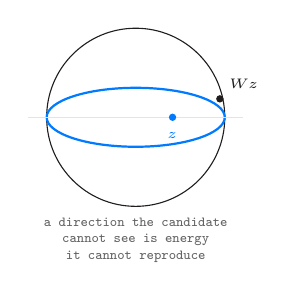
\begin{tikzpicture}[scale=0.78]
        \draw[ink] (0,0) circle (1.45);
        \draw[accent,thick] (0,0) ellipse (1.45 and 0.48);
        \draw[hairline] (-1.75,0) -- (1.75,0);
        \fill[ink] (1.37,0.30) circle (1.7pt);
        \node[font=\ttfamily\tiny,color=ink,above right] at (1.37,0.30) {$Wz$};
        \fill[accent] (0.6,0) circle (1.7pt);
        \node[font=\ttfamily\tiny,color=accent,below] at (0.6,-0.08) {$z$};
        \node[font=\ttfamily\tiny,color=mute,align=center] at (0,-2.0)
          {a direction the candidate\\cannot see is energy\\it cannot reproduce};
      \end{tikzpicture}
    \end{column}
  \end{columns}
\end{frame}

% ============================================================== 06 spectra
\begin{frame}{Act two: what do trained matrices look like?}
  \vspace{2pt}
  \begin{center}
    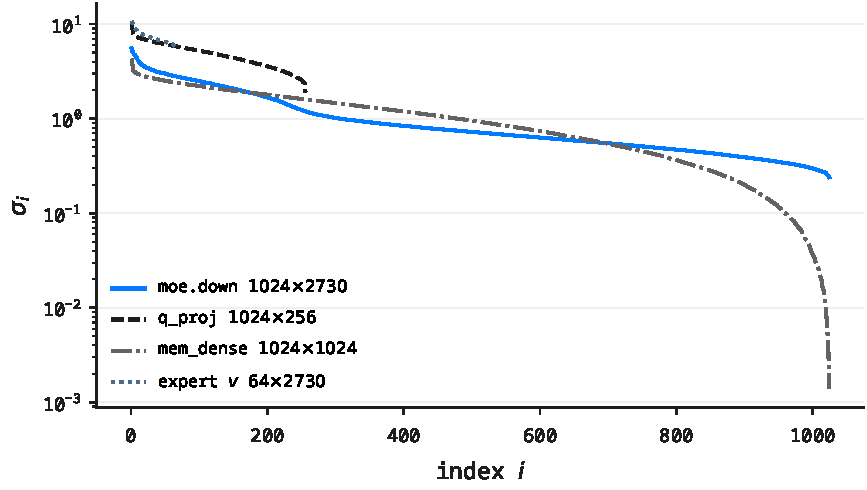
\includegraphics[width=0.88\textwidth]{figures/spectrum.pdf}
  \end{center}
  \vspace{-2pt}
  {\ttfamily\scriptsize\color{stone}
  four matrices from one checkpoint\quad·\quad five orders of magnitude\quad·\quad
  not one of them snaps to zero}
\end{frame}

% ============================================================== 07 surprise (dark)
{
\setbeamertemplate{background canvas}{\color{dark}\vrule width\paperwidth height\paperheight}
\setbeamercolor{normal text}{fg=canvas}
\setbeamertemplate{footline}{%
  \hspace*{14pt}{\ttfamily\tiny\color{darkelev}the rank of a matrix, and what it costs}\hfill
  {\ttfamily\tiny\color{on-dark-mute}\insertframenumber\,/\,10}\hspace*{14pt}\vspace{6pt}}
\definecolor{on-dark-mute}{HTML}{9A9898}
\begin{frame}{The expectation fails}
  \vspace{2pt}
  \begin{columns}[T]
    \begin{column}{0.50\textwidth}
      \includegraphics[width=\textwidth]{figures/mass_dark.pdf}
    \end{column}
    \begin{column}{0.46\textwidth}
      {\ttfamily\scriptsize\color{on-dark-mute}
      \begin{tabular}{@{}lr@{}}
        \toprule
        matrix & mass at $r{=}64$ \\
        \midrule
        moe.down    & 41\% \\
        q\_proj      & 45\% \\
        mem\_dense   & \bad{28\%} \\
        expert $v$   & 100\% \\
        \bottomrule
      \end{tabular}}

      \vspace{12pt}
      {\small\color{canvas}
      Trained matrices are \bad{not} nearly low-rank.\par}

      \vspace{6pt}
      {\small\color{on-dark-mute}
      Truncating a trained layer to rank 64 throws away more than half of it by
      the theorem's own measure. The last row is different for a structural
      reason --- next slide.\par}
    \end{column}
  \end{columns}
\end{frame}
}

% ============================================================== 08 resolution
\begin{frame}{Compression is not reparameterisation}
  \vspace{2pt}
  {\small\color{bodyink}
  The expert matrix is rank 64 \hl{by construction}: we never store a
  $64\times2730$ matrix, we store two thin ones whose product has rank $\le64$.\par}

  \[
    W = U V^{\top},\qquad U\in\mathbb{R}^{64\times64},\; V\in\mathbb{R}^{64\times2730}
  \]

  \vspace{2pt}
  \begin{columns}[T]
    \begin{column}{0.47\textwidth}
      \vspace{2pt}
      {\ttfamily\scriptsize\color{stone}COMPRESSION}\\[3pt]
      {\small\color{bodyink}
      Given a fixed $W$, how well can rank $r$ imitate it?\par}
      \vspace{3pt}
      {\color{danger}\ttfamily\small answer: badly}
    \end{column}
    \begin{column}{0.47\textwidth}
      \vspace{2pt}
      {\ttfamily\scriptsize\color{stone}REPARAMETERISATION}\\[3pt]
      {\small\color{bodyink}
      Restrict the layer to rank $r$ before training, and let descent search
      inside that family.\par}
      \vspace{3pt}
      {\color{success}\ttfamily\small answer: almost free}
    \end{column}
  \end{columns}

  \vspace{10pt}
  {\color{bodyink}
  Eckart--Young bounds the first. It says \hl{nothing} about the second --- and
  the second is what gets deployed.\par}
\end{frame}

% ============================================================== 09 price
\begin{frame}{The price, measured}
  \begin{columns}[T]
    \begin{column}{0.52\textwidth}
      \vspace{4pt}
      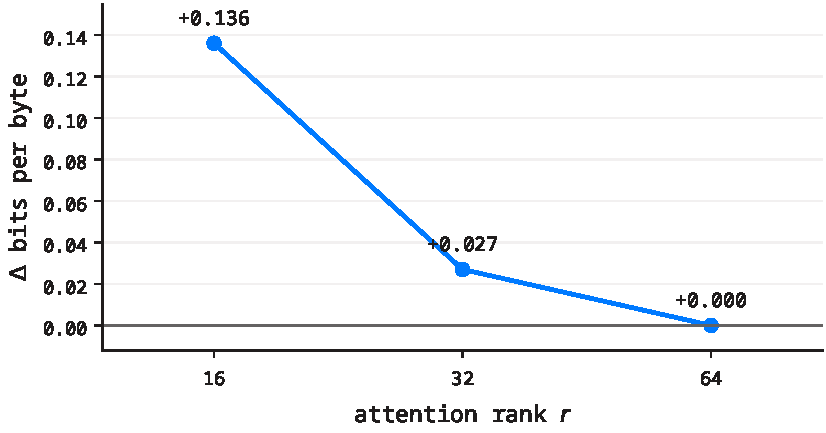
\includegraphics[width=\textwidth]{figures/rank_ladder.pdf}
    \end{column}
    \begin{column}{0.44\textwidth}
      \vspace{2pt}
      {\ttfamily\scriptsize\color{stone}THREE SEEDS per arm · identical budget}\\[6pt]
      {\ttfamily\small
      \begin{tabular}{@{}lrr@{}}
        \toprule
        rank & $\Delta$ bits/byte & storage \\
        \midrule
        64 & baseline   & $1.00\times$ \\
        32 & $+0.027$   & $0.50\times$ \\
        16 & $+0.136$   & $0.25\times$ \\
        \bottomrule
      \end{tabular}}

      \vspace{10pt}
      {\small\color{bodyink}
      Halving the rank costs about $2\%$ of quality; quartering it costs $10\%$.\par}

      \vspace{6pt}
      {\small\color{bodyink}
      The spectrum predicts the \emph{shape} of this curve. Only the experiment
      gives its \hl{height}.\par}
    \end{column}
  \end{columns}
\end{frame}

% ============================================================== 10 takeaway
\begin{frame}{Three things to take away}
  \vspace{4pt}
  \begin{itemize}\itemsep10pt
    \item \hl{a matrix is a shape} --- the singular values are its semi-axes, and
          the truncated SVD is the optimal rank-$r$ replacement, with the error
          known in advance
    \item \hl{trained matrices are not low-rank} --- measured: rank 64 keeps
          28--45\% of the mass; the naive compression story is false for real weights
    \item \hl{compress $\ne$ reparameterise} --- truncating is expensive,
          training inside the family is nearly free, and only the first is
          covered by the theorem
  \end{itemize}

  \vspace{10pt}
  {\color{hairline}\rule{\textwidth}{0.6pt}}
  \vspace{6pt}
  {\ttfamily\scriptsize\color{stone}
  exercise\quad take any layer, compute $\sigma_i$, predict the loss after
  truncation with $\sqrt{\sum_{i>r}\sigma_i^2}$, then measure.\\
  \hspace*{2.9em}the ratio between prediction and reality is the interesting number.}
\end{frame}

\end{document}
